\documentclass[11pt,letterpaper]{report}
\usepackage[margin=1in]{geometry}
\usepackage[latin1]{inputenc}
\usepackage{url}
\usepackage{hyperref}
\usepackage{doi}
\usepackage{breakurl}
\urlstyle{same} 			% Use same font type and size for url as the text.

\usepackage{natbib}
\usepackage{fancyhdr}
\pagestyle{fancy}
\usepackage[hang]{footmisc}
\usepackage[textfont={bf}]{caption}
\usepackage{amsmath}
\usepackage{amsfonts}
\usepackage{amssymb}
\usepackage{graphicx}
\usepackage[version=3]{mhchem}
\usepackage[table,usenames,dvipsnames,svgnames,x11names]{xcolor}
\usepackage{color}
\usepackage{dcolumn}
\usepackage{booktabs}
\usepackage{pdflscape}
\usepackage{textcomp}
\usepackage{float}
\usepackage{subfig}
\usepackage{chngcntr}
\usepackage{needspace}
\counterwithout{figure}{chapter}
%\usepackage[usenames,dvipsnames,svgnames]{xcolor}
\definecolor{darkerGreen}{rgb}{0.702,0.800,0.510}
\definecolor{darkGreen}{rgb}{0.839,0.890,0.737}
\definecolor{liteGreen}{rgb}{0.918,0.945,0.867}
\definecolor{lightgray}{gray}{0.9}
\definecolor{lightblue}{rgb}{0.93,0.95,1.0}
\definecolor{URLBlue}{rgb}{0,0,0.5} % Define new color for hyperlinks
\hypersetup{
	colorlinks   = true,
	citecolor    = URLBlue,
	linkcolor    = URLBlue,
	urlcolor     = URLBlue
}

\definecolor{TableBorder}{rgb}{0.325,0.557,0.835}
%\definecolor{TableEven}{rgb}{0.8000,0.9216,0.9490}
\definecolor{TableEven}{rgb}{0.773,0.851,0.945}
\definecolor{TableOdd}{rgb}{1,1,1}

%\usepackage{pstricks,pst-node,pst-tree}

\usepackage{pgfplots}
\usetikzlibrary{matrix}
\usepgfplotslibrary{groupplots}

\pgfplotsset{compat=newest}
\pgfplotsset{every axis/.append style={line width=0.75pt},
   axis x line*=bottom, axis y line*=left}
\pgfsetplotmarksize{0pt}

\usetikzlibrary{shapes,arrows}
% Define block styles
\tikzstyle{decision} = [diamond, draw, fill=blue!20,
   text width=5.0em, text badly centered, node distance=3cm, inner sep=0pt]
\tikzstyle{block} = [rectangle, draw, fill=blue!20,
   minimum width=5cm, minimum height=2.0cm, text centered, text width=5cm,
   rounded corners, minimum height=4em]
\tikzstyle{smallblock} = [rectangle, draw, fill=blue!20,
   minimum width=2.5cm, minimum height=2.0cm, text centered, text width=2.5cm,
   rounded corners, minimum height=4em]
\tikzstyle{line} = [draw, -latex']
\tikzstyle{cloud} = [draw, ellipse,fill=red!20, node distance=5cm, minimum height=1.5cm]
\usepackage{tikzpagenodes}
\usetikzlibrary{calc}
\definecolor{GTAPBlue}{RGB}{27,66,115}
\definecolor{GTAPOrange}{RGB}{243,143,34}

\usepackage{forest}
\usetikzlibrary{shadows}
% RGB scale relative to 255
\definecolor{TableBorder}{rgb}{0.325,0.557,0.835}
%\definecolor{TableEven}{rgb}{0.8000,0.9216,0.9490}
\definecolor{TableEven}{rgb}{0.773,0.851,0.945}
\definecolor{TableOdd}{rgb}{1,1,1}
\newcommand\VRule[1][\arrayrulewidth]{\vrule width #1}
\definecolor{dkBlue}{rgb}{0.6157 0.7647 0.9020}
\definecolor{mdBlue}{rgb}{0.7412 0.8431 0.9333}
\definecolor{ltBlue}{rgb}{0.8706 0.9216 0.9686}

\begin{document}

\section{Knowledge module: core theory}

[NEW 20-JAN-2019] The model includes a knowledge
module that operates somewhat similarly to investment
and the capital stock. Each year there is aggregate expenditure
on research and development (R\&D), that is captured
by the variable $\mathit{XFD}_{\mathit{r\_d}}$. This
expenditure flow increases knowledge, though knowledge
also depreciates each year. The main difference
with the usual capital/investment dynamic,
is that the impact
of R\&D expenditures happens with a distributed lag.\footnote{This
formulation is inspired by \cite{SmeetsKristkova2016}.}
The latter is governed by a \emph{Gamma} distribution
function, the parameters and length of which
are region specific.\footnote{Additional details
and example distribution functions are provided
in Annex~\ref{sec:knowledge}.}

Equation~(\ref{eq:kn}) describes the motion equation for knowledge.
The variable $\mathit{KN}$ represents
the stock of knowledge. It is equal to the previous
period's knowledge stock---adjusted by depreciation, $\delta^k$---,
plus the distributed lag of current
and previous expenditures on R\&D, where $\gamma^k$
represents the lag coefficients.\footnote{If
$\gamma^k_0=0$ and $\gamma^k_{1}=1$, the equation
would have the same assumption as the standard
capital accumulation equation.}
Annex~\ref{sec:knowledge} describes how the
model implements the knowledge module. Implementation
requires taking into account two features. (1) It is implemented
using the variable time step that is a central
part of the model. Because of the distributed
lags, this also requires that the R\&D expenditures
be evaluated each \emph{year}, independently of
the time step. (2) The first years of the simulation require
a backward projection of the R\&D expenditures,
i.e. prior to the initial year. If $N$ is 50
for example, it requires projecting R\&D
expenditures back some 50 years.

\begin{equation}
\label{eq:kn}
\mathit{KN}_{r,t} = \left(1-\delta^k_r \right) \mathit{KN}_{r,t-1}
+ \sum_{i=0}^N{\gamma^k_{r,i} \mathit{XFD}_{r,\mathit{r\_d},t-i}}
\end{equation}

\noindent where
\[
\gamma^k_{i} = \chi \left(i + 1 \right)^{\delta/(1-\delta)}\lambda^i
\]

In its default mode, the user inputs R\&D expenditures as
a (percent) share of reference year GDP. The default closure
fixes the (real) GDP share of R\&D expenditures at the reference
year level. The model specification assumes that R\&D expenditures
are paid for from government revenues.

The knowledge module is designed to impact on labor
productivity growth. Equation~(\ref{eq:pik}) describes the relation
between the endogenous component of labor productivity
in sector $a$, $\pi^k$, relative to the growth rate of the stock
of knowledge. The elasticity is given by $\epsilon^r$ and
is allowed to be sector specific. The shifter, $\gamma^r$, is initialized
at 1.

\begin{equation}
\label{eq:pik}
\pi^k_{r,a,t} = \gamma^r_{r,a,t} \epsilon^r_{r,a,t}
\left(\frac{\mathit{KN}_{r,t}}{\mathit{KN}_{r,t-1}} - 1\right)
\end{equation}

\section{Knowledge module: implementation}
\label{sec:knowledge}

The starting point for the model implementation is the 1-step
motion equation for the knowledge stock\footnote{In the 
model the variable $\mathit{RD}$ is given by 
$\mathit{XFD}_{\mathit{rd}}$.}:

\[
\mathit{KN}_{t} = \left(1-\delta \right) \mathit{KN}_{t-1}
+ \sum_{k=0,i=t}^{N,t-N}{\gamma_k \mathit{RD}_{i}} = \left(1-\delta \right) \mathit{KN}_{t-1} + G'\mathit{RDL}_{t,t}
\]

\noindent where the last term is the summation expression in vector
form (the double-indexed subscript will become clearer below). $G'\mathit{RDL}$
represents the gamma-weighted sum of the lags of R\&D expenditures.
From this, we can use induction and convert the one-step expression to
an $n$-step expression, equation~(\ref{eq:knmod}). The first term
on the right-hand side is intuitive. The second term adds all
of the relevant cumulative weighted-lags and includes the
appropriate depreciation for the intermediate years. Say for example
we are evaluating knowledge stock in year 2025 with respect to 2020. The
sum will be over all years between 2021 and 2025 inclusive.
Equation~(\ref{eq:rdl}) calculates the cumulative weighted
lags for each year between $t-n+1$ and $t$, e.g. between
2021 and 2025 for the example above. It does require, nonetheless, the level of R\&D 
expenditures for the intermediate years. Since these have differing weights
over time, we need to keep track of these explicitly.
In the GAMS code, most equations are indexed over $t$,
which has variable step sizes. The R\&D variable is
calculated for each year, assuming constant growth
in the intermediate years. Equation~(\ref{eq:rdgr})
determines the multi-step growth rate. Equation~(\ref{eq:rd1})
defines R\&D expenditures for each year, irrespective
of the model's time step.

\begin{equation}
\label{eq:knmod}
\mathit{KN}_{t} = \left( 1 - \delta \right)^n \mathit{KN}_{t-n}
+ \sum_{i=t-n+1}^{t}{\left( 1 - \delta \right)^{t-i} \mathit{RDL}_{i,t}}
\end{equation}

\begin{equation}
\label{eq:rdl}
\mathit{RDL}_{i,t} = \sum_{k=0, j=i-k}^{N,i-N}{\gamma_k \mathit{RD}_j}
\qquad \textrm{for } t-n<i \le t
\end{equation}

\begin{equation}
\label{eq:rdgr}
\mathit{RD}_{t} = \left( 1 + \mathit{gr}_t \right)^{n}
\mathit{RD}_{t-n}
\end{equation}

\begin{equation}
\label{eq:rd1}
\mathit{RD}_{i} = \left( 1 + \mathit{gr}_t \right)^{n-(t-i)}
\mathit{RD}_{t-n} \qquad \textrm{for } t-n<i<t
\end{equation}

In the model implementation, a macro is used to substitute
equation~(\ref{eq:rdl}) into equation~(\ref{eq:knmod}).
And equations~(\ref{eq:rdgr}) and~(\ref{eq:rd1}) can be collapsed to equation~(\ref{eq:rd})
thereby eliminating the growth rate of R\&D expenditures, where
the calculations are done for each year between $t-n$ and $t$.

\begin{equation}
\label{eq:rd}
\mathit{RD}_{i} = \mathit{RD}_{t-n}^{(t-i)/n}
\mathit{RD}_{t}^{(n-(t-i))/n} \qquad \textrm{for } t-n<i<t
\end{equation}

If R\&D is growing at a steady rate of $g$, we can then write:

\begin{equation}
\label{eq:knss}
\begin{array} {l c l}
\mathit{KN}_{t} & = & \displaystyle \left(1-\delta \right) \mathit{KN}_{t-1}
+ \sum_{k=0}^N{\gamma_{k} \mathit{RD}_{t-N} \left(1+g\right)^{N-k}} \\
{}  & = & \displaystyle \left(1-\delta \right) \mathit{KN}_{t-1}
+ \mathit{RD}_{t} \sum_{k=0}^N{ \frac{\gamma_{k}}{\left(1+g\right)^k} } \\
\end{array}
\end{equation}

\noindent In steady state, the summation term is a constant and we can
thus write:

\[
\mathit{KN}_{t} = \displaystyle \left(1-\delta \right) \mathit{KN}_{t-1}
+ \beta \mathit{RD}_{t} \qquad \textrm{where } \beta = \displaystyle \sum_{k=0}^N{ \frac{\gamma_{k}}{\left(1+g\right)^k} }
\]

\noindent The formula can also be converted to work with multi-year time steps.

\[
\begin{array}{l c l}
\mathit{KN}_{t}
& = & \displaystyle \left(1-\delta \right) \mathit{KN}_{t-1} + \beta \mathit{RD}_{t} \\
{} & = & \displaystyle \left(1-\delta \right) \left[\left(1-\delta \right) \mathit{KN}_{t-2} + \beta \mathit{RD}_{t-1} \right] + \beta \mathit{RD}_{t} \\
{} & = & \displaystyle \left(1-\delta \right)^2 \mathit{KN}_{t-2} + \left(1-\delta \right) \beta \mathit{RD}_{t-1} + \beta \mathit{RD}_{t} \\
{} & = & \displaystyle \left(1-\delta \right)^3 \mathit{KN}_{t-3} + \left(1-\delta \right)^2 \beta \mathit{RD}_{t-2} + \left(1-\delta \right) \beta \mathit{RD}_{t-1} + \beta \mathit{RD}_{t} \\
{} & \vdots & {} \\
{} & = & \displaystyle \left(1-\delta \right)^n \mathit{KN}_{t-n} + \beta \sum_{i=0}^{n-1}{\left(1-\delta \right)^i  \mathit{RD}_{t-i}} \\
\end{array}
\]\

\noindent Assuming a constant growth rate for R\&D expenditures, the last expression becomes:
\[
\mathit{KN}_{t} = \displaystyle \left(1-\delta \right)^n \mathit{KN}_{t-n} + \beta \sum_{i=0}^{n-1}{\left(1-\delta \right)^i  \mathit{RD}_{t} \left(1+g\right)^{-i}}
\]

\noindent where
\[
\mathit{RD}_{t} = \mathit{RD}_{t-i}  \left(1+g\right)^{i}
\]

\noindent After a bit of algebra, it is straightforward to show that the summation expression simplifies to:

\[
\sum_{i=0}^{n-1}{\frac{\left(1-\delta \right)^i} {\left(1+g\right)^{i}}} = \frac{1}{\left( 1 + g\right)^{n-1}}
\frac{\left(1+g\right)^n - \left(1-\delta\right)^n}{g + \delta}
\]

\noindent The final expression can thus be written as:
\[
\begin{array}{l c l}
\mathit{KN}_{t} & = & \displaystyle \left(1-\delta \right)^n \mathit{KN}_{t-n} + \beta \frac{\mathit{RD}_{t}}{\left( 1 + g\right)^{n-1}} \frac{\left(1+g\right)^n - \left(1-\delta\right)^n}{g + \delta} \\
& = & \displaystyle \left(1-\delta \right)^n \mathit{KN}_{t-n} + {\beta\left( 1 + g\right)\mathit{RD}_{t-n}} \frac{\left(1+g\right)^n - \left(1-\delta\right)^n}{g + \delta} \\
\end{array}
\]

These formulas rely on $n > N$, or that that the growth rate is uniform back through period $t-N$.

From the last formula, we can show that in steady-state the following
relation must hold for the ratio of knowledge stocks relative to R\&D expenditures:

\[
\frac{\mathit{KN}} {\mathit{RD}} = \beta \frac{1+g}{g+\delta}
\]

\subsection*{Implementation}

Initializing the stock of knowledge and the pre-base year R\&D expenditures
is an issue. The strategy followed so far is based on the following steps:

\begin{itemize}
	\item {Assume a given base year level of R\&D. Calculate
		the knowledge stock ($\mathit{KN}$) expenditure consistent with some assumption about the steady-state
		growth rate around the base year and the rate of knowledge depreciation.
		From the expression above, we have:
		\[{\mathit{KN}_{t_0}} = {\beta}  {\mathit{RD}_{t_0}}\frac{1+g}{g+\delta} =
		{\mathit{RD}_{t_0}} \frac{1+g}{g+\delta}\displaystyle \sum_{k=0}^N{ \frac{\gamma_{k}}{\left(1+g\right)^k} }
		\] Alternatively, one could make an assumption about the base
		year knowledge stock and invert the expression to calculate the
		R\&D expenditures consistent with the steady-state assumption.}
	\item {Back-cast the R\&D expenditures to the earliest period, that
		should be at least $N$ years back or more, for the largest $N$:
		\[
		\mathit{RD}_t = \mathit{RD}_{t+1} / \left(1+g\right) \qquad
		\textrm{for } t_f \le t < t_0-1
		\]
		where $t_f$ is the first year defined, e.g. 1960, and
		$t_0$ is the base year for the simulations, e.g. 2014.}
	\item {Back-cast the cumulative lag structure, $\mathit{RDL}$ using the following formula:
		\[
		\mathit{RDL}_{t,t_0}
		\sum_{k=0, i=t-k}^{N,t-N}{\gamma_{k}\mathit{RD}_i}
		\qquad \textrm{for } t_f+N \le t \le t_0
		\]}
	\item {Back-cast the stock of knowledge. This step is
		not strictly necessary.
		\[
		\mathit{KN}_t = \frac{\mathit{KN}_{t+1} - \mathit{RDL}_{t+1,t_0}}
		{1-\delta} \qquad \textrm{for } t_f+N-1 \le t < t_0
		\]}
	
\end{itemize}

\begin{figure}[ht]
	\centering
	\subfloat[][$\delta=0.7$, \scriptsize{$\lambda=0.9$, $N=50$, max=21.1, mean=25.8}]{
		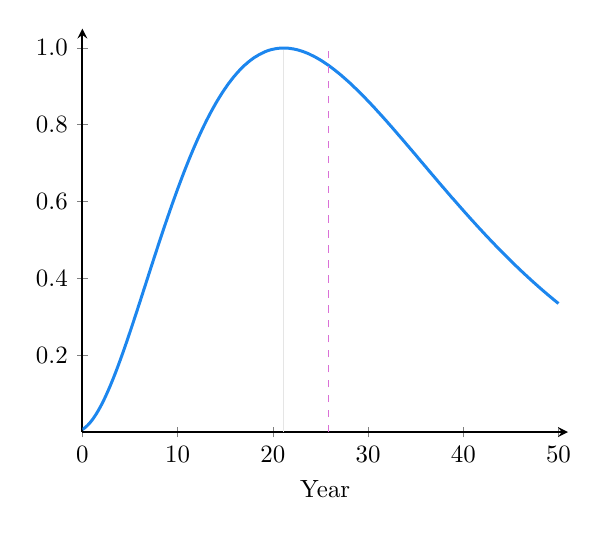
\begin{tikzpicture}[scale=0.9]
		\begin{axis}[axis x line=bottom, axis y line=left, xlabel=Year,
		xtick={0,10,...,50}, ytick={0.2,0.4,...,1.0}, xmax=51, ymax=1.05,
		y tick label style={/pgf/number format/.cd,fixed,fixed zerofill,precision=1,/tikz/.cd}]
		\addplot[DodgerBlue2,very thick,mark=none,domain=0:50,samples=501]
		{0.006738536*exp(0.7*ln(\x+1)/(1-0.7) + \x*ln(0.9))};
		\addplot[lightgray,thin,mark=none]
		coordinates{(21.1,0) (21.1,0.995)} ;
		\addplot[Orchid,thin,dashed,mark=none]
		coordinates{(25.8,0) (25.8,1)} ;
		\end{axis}
		\end{tikzpicture}
	} \qquad
	\subfloat[][$\delta=0.7$, \scriptsize{$\lambda=0.8$, $N=35$, max=9.5, mean=13.4}]{
		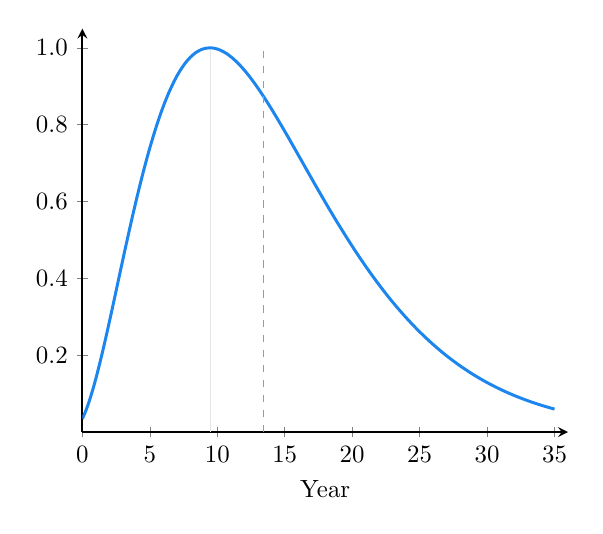
\begin{tikzpicture}[scale=0.9]
		\begin{axis}[axis x line=bottom, axis y line=left, xlabel=Year,
		xtick={0,5,...,35}, ytick={0.2,0.4,...,1.0}, xmax=36, ymax=1.05,
		y tick label style={/pgf/number format/.cd,fixed,fixed zerofill,precision=1,/tikz/.cd}]
		\addplot[DodgerBlue2,very thick,mark=none,domain=0:35,samples=351]
		{0.03450336*exp(0.7*ln(\x+1)/(1-0.7) + \x*ln(0.8))};
		\addplot[lightgray,thin,mark=none]
		coordinates{(9.5,0) (9.5,0.995)} ;
		\addplot[Orchid,thin,dashed,mark=none]
		coordinates{(13.4,0) (13.4,1)} ;
		\end{axis}
		\end{tikzpicture}
	} \\
	\subfloat[][$\delta=0.6$, \scriptsize{$\lambda=0.85$, $N=25$, max=8.2, mean=11.6}]{
		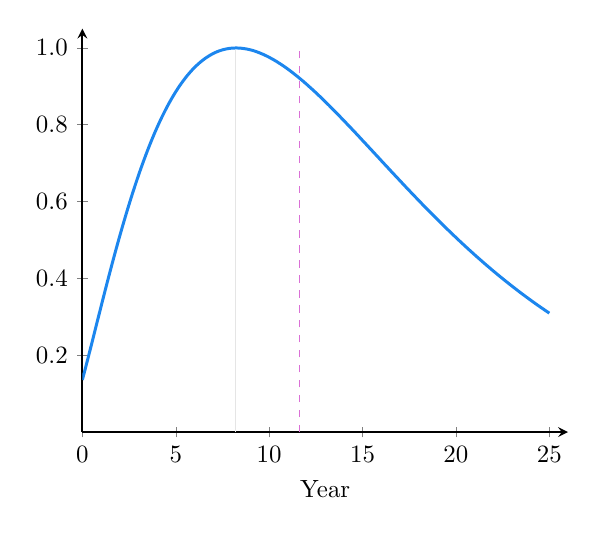
\begin{tikzpicture}[scale=0.9]
		\begin{axis}[axis x line=bottom, axis y line=left, xlabel=Year,
		xtick={0,5,...,25}, ytick={0.2,0.4,...,1.0}, xmax=26, ymax=1.05,
		y tick label style={/pgf/number format/.cd,fixed,fixed zerofill,precision=1,/tikz/.cd}]
		\addplot[DodgerBlue2,very thick,mark=none,domain=0:25,samples=251]
		{0.135856271*exp(0.6*ln(\x+1)/(1-0.6) + \x*ln(0.85))};
		\addplot[lightgray,thin,mark=none]
		coordinates{(8.2,0) (8.2,0.995)} ;
		\addplot[Orchid,thin,dashed,mark=none]
		coordinates{(11.6,0) (11.6,1)} ;
		\end{axis}
		\end{tikzpicture}
	} \qquad
	\subfloat[][$\delta=0.4$, \scriptsize{$\lambda=0.8$, $N=15$, max=2.0, mean=5.4}]{
		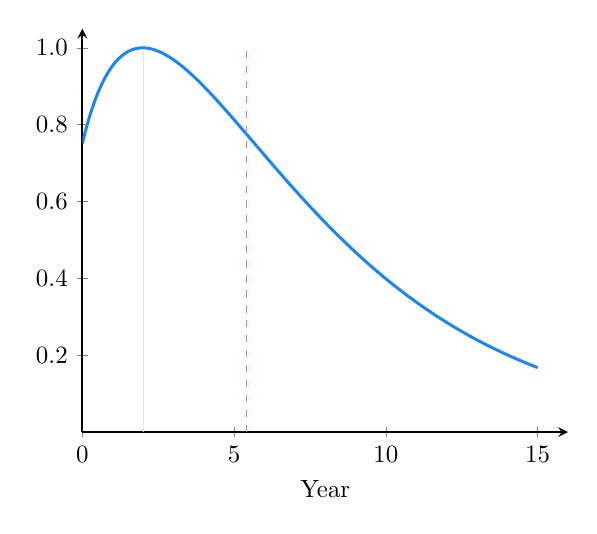
\begin{tikzpicture}[scale=0.9]
		\begin{axis}[axis x line=bottom, axis y line=left, xlabel=Year,
		xtick={0,5,...,15}, ytick={0.2,0.4,...,1.0}, xmax=16, ymax=1.05,
		y tick label style={/pgf/number format/.cd,fixed,fixed zerofill,precision=1,/tikz/.cd}]
		\addplot[DodgerBlue2,very thick,mark=none,domain=0:15,samples=151]
		{0.751167359*exp(0.4*ln(\x+1)/(1-0.4) + \x*ln(0.8))};
		\addplot[lightgray,thin,mark=none]
		coordinates{(2.0,0) (2.0,0.995)} ;
		\addplot[Orchid,thin,dashed,mark=none]
		coordinates{(5.4,0) (5.4,1)} ;
		\end{axis}
		\end{tikzpicture}
	} \\
	\subfloat[][$\delta=0.7$, \scriptsize{$\lambda=0.9$, $N=25$, max=21.1, mean=16.3}]{
		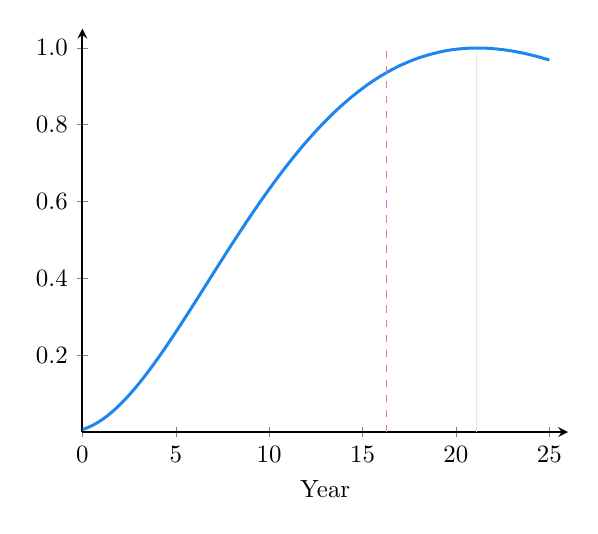
\begin{tikzpicture}[scale=0.9]
		\begin{axis}[axis x line=bottom, axis y line=left, xlabel=Year,
		xtick={0,5,...,25}, ytick={0.2,0.4,...,1.0}, xmax=26, ymax=1.05,
		y tick label style={/pgf/number format/.cd,fixed,fixed zerofill,precision=1,/tikz/.cd}]
		\addplot[DodgerBlue2,very thick,mark=none,domain=0:25,samples=251]
		{0.006738536*exp(0.7*ln(\x+1)/(1-0.7) + \x*ln(0.9))};
		\addplot[lightgray,thin,mark=none]
		coordinates{(21.1,0) (21.1,0.99)} ;
		\addplot[Orchid,thin,dashed,mark=none]
		coordinates{(16.3,0) (16.3,1)} ;
		\end{axis}
		\end{tikzpicture}
	} \qquad
	\subfloat[][$\delta=0.5$, \scriptsize{$\lambda=0.8$, $N=15$, max=3.5, mean=6.3}]{
		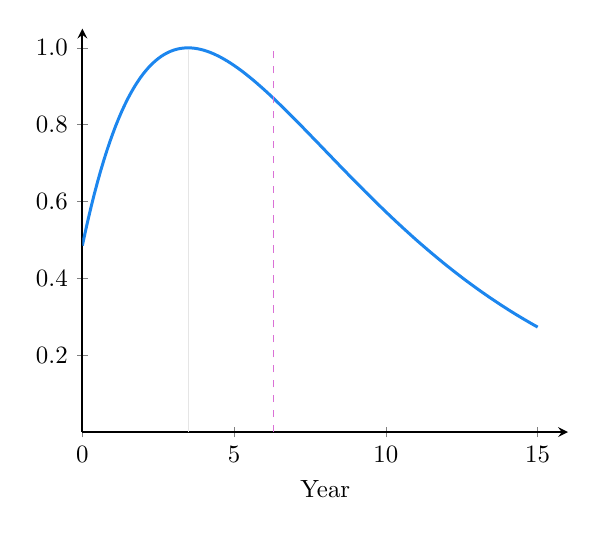
\begin{tikzpicture}[scale=0.9]
		\begin{axis}[axis x line=bottom, axis y line=left, xlabel=Year,
		xtick={0,5,...,15}, ytick={0.2,0.4,...,1.0}, xmax=16, ymax=1.05,
		y tick label style={/pgf/number format/.cd,fixed,fixed zerofill,precision=1,/tikz/.cd}]
		\addplot[DodgerBlue2,very thick,mark=none,domain=0:15,samples=151]
		{0.48525365*exp(0.5*ln(\x+1)/(1-0.5) + \x*ln(0.8))};
		\addplot[lightgray,thin,mark=none]
		coordinates{(3.5,0) (3.5,0.995)} ;
		\addplot[Orchid,thin,dashed,mark=none]
		coordinates{(6.3,0) (6.3,1)} ;
		\end{axis}
		\end{tikzpicture}
	} \\
	\caption{Gamma distribution examples}
	\label{fig:gamDist}
\end{figure}

%\bibliographystyle{../../../Word/Latex/JGEA/JGEA}
\bibliography{../../../Bib/vdMRef}

\begin{verbatim}
@Article{SmeetsKristkova2016,
  author   = {Zuzana {Smeets {K\v{r}\'istkov\'a}} and Michiel {van Dijk} and Hans {van Meijl}},
  journal  = {{NJAS} - Wageningen Journal of Life Sciences},
  title    = {Projections of long-term food security with {R\&D} driven technical change---A {CGE} analysis},
  year     = {2016},
  issn     = {1573-5214},
  pages    = {39--51},
  volume   = {77},
  abstract = {In this paper, the impact of public {R\&D} investment on agricultural productivity and
 long-term food security via {R\&D} driven endogenous technical change is analysed.
 The findings show that {R\&D} growth rates at the level reached in 2000s, particularly those for
 China, would not be expected any longer. Concerning the impact of projected {R\&D} investments on
 agricultural productivity, it is found that endogenous growth rates of land-augmenting technical
 change are comparably lower than the standard exogenous rates used in long term projections
 of agri-food markets. This suggests that public {R\&D} investments are not able to stimulate
 agricultural production to the levels that would be expected from the standard baseline outcomes.},
  doi      = {10.1016/j.njas.2016.03.001},
  keywords = {Public agricultural {R\&D}, investment, Land-augmenting technical change, Agricultural productivity, CGE model, {MAGNET}, Food security},
} 
\end{verbatim}

\end{document}